\documentclass[12pt]{book}
\title{Eigenmath Manual}
\author{George Weigt}
\date{May 17, 2007}
\usepackage{graphicx}

\begin{document}
\maketitle
\tableofcontents

\newpage

\chapter{The Big Picture}
In simplest terms, when you type something into Eigenmath,
it gets evaluated and typically a result is printed.
For a first example, try entering $1/2+1/3$.

\medskip
\verb$1/2+1/3$
$$5\over6$$

\medskip
\noindent
As you can see, Eigenmath uses rational arithmetic for numerical calculations.
You can enter $float$ to convert the result to a floating point number.

\medskip
\verb$float$
$$0.833333$$

\medskip
\noindent
There are a number of features for doing symbolic calculations.
Here is a preview.

\medskip
\verb$integral(log(x))$
$$-x+x\log(x)$$

\newpage

\noindent
This table summarizes Eigenmath's input syntax.
The symbol {\tt\char32} indicates a mandatory space.

\begin{center}
\begin{tabular}{clll}
$-a$ & & {\tt -a} \\
\\
$a+b$ & & {\tt a+b} \\
\\
$a-b$ & & {\tt a-b} \\
\\
$ab$ & & {\tt a*b} & {\tt a{\char32}b} \hspace{10pt} {\it alternate form}\\
\\
$\displaystyle{a\over b}$ & & {\tt a/b} \\
\\
$\displaystyle{a\over bc}$ & & {\tt a/b/c} \\
\\
$a^2$ & & {\tt a{\char94}2} \\
\\
$\sqrt{a}$ & & {\tt a{\char94}(1/2)} & {\tt sqrt(a)} \\
\\
$\displaystyle{1\over\sqrt a}$ & & {\tt a{\char94}(-1/2)} & {\tt 1/sqrt(a)} \\
\\
$a(b+c)$ & & {\tt a*(b+c)} & {\tt a{\char32}(b+c)} \\
\\
$f(a)$ & & {\tt f(a)} \\
\\
$\displaystyle{\left(\matrix{a\cr b\cr c\cr}\right)}$ & & {\tt (a,b,c)} \\
\\
$\displaystyle{\left(\matrix{a&b\cr c&d\cr}\right)}$ & & {\tt ((a,b),(c,d))} \\
\\
 & & {\tt T[1]} & {\it tensor component access} \\
\\
 & & {\tt T[1,2]} \\
\end{tabular}
\end{center}

\newpage

\noindent
A geometric series converges according to the formula
$$\sum_{k=0}^\infty a^k={1\over1-a},\qquad|a|<1$$
If we use $a=-1/2$ and for practical purposes only count up to nine instead of infinity,
we should have
$$\sum_{k=0}^9\left(-{1\over2}\right)^k\approx{2\over3}$$
In the following examples, various Eigenmath features will be demonstrated
by computing this formula in different ways.

\medskip
\noindent
To begin, here is the calculation in one line of code.

\medskip
\verb$sum(k,0,9,(-0.5)^k)$
$$0.666016$$

\medskip
\noindent
The following example uses an intermediate variable.

\medskip
\verb$f=sum(k,0,9,a^k)$

\verb$f$
$$f=1+a+a^2+a^3+a^4+a^5+a^6+a^7+a^8+a^9$$

\verb$eval(f,a,-1/2)$
$$341\over512$$

\verb$float(last)$
$$0.666016$$

\medskip
\noindent
As seen on the first line, no result is printed when a symbol is defined.
When you do in fact want to see the value of a symbol,
just enter it as shown on the second line.

\medskip
\noindent
When a result is displayed, it is also stored in the symbol $last$.

\newpage

\noindent
The following example shows how to define a function.

\medskip
\verb$f(a)=sum(k,0,9,a^k)$

\verb$f$
$$f=\mathop{\rm sum}(k,0,9,a^k)$$

\verb$f(-1/2)$
$$341\over512$$

\verb$f(-0.5)$
$$0.666016$$

\medskip
\noindent
Eigenmath handles function definitions in a special way.
Unlike a normal symbol, a function definition is not evaluated immediately.
The following example demonstrates the difference.

\medskip
\verb$f=sum(k,0,9,a^k)$

\verb$f$
$$f=1+a+a^2+a^3+a^4+a^5+a^6+a^7+a^8+a^9$$

\verb$f(a)=sum(k,0,9,a^k)$

\verb$f$
$$f=\mathop{\rm sum}(k,0,9,a^k)$$

\medskip
\noindent
Why are they handled differently?
Well, suppose you want to define $f$ as a function of two variables, $a$ and $n$, like this.

\medskip
\verb$f(a,n)=sum(k,0,n,a^k)$

\medskip
\noindent
In this case it is not possible to evaluate the sum right away.
The value of $n$ will not be known until $f$ is actually used somewhere.
Consequently, Eigenmath does not normally evaluate a function when it is defined.
Now, having said that, there are two work arounds that provide exceptions to the rule.
They are {\it eval} and {\it quote}.
 
\medskip
\verb$f=quote(sum(k,0,9,a^k))$

\verb$f$
$$f=\mathop{\rm sum}(k,0,9,a^k)$$

\verb$f(a)=eval(sum(k,0,9,a^k))$

\verb$f$
$$f=1+a+a^2+a^3+a^4+a^5+a^6+a^7+a^8+a^9$$

\newpage

\chapter{Scripting}

\noindent
Here is a simple example that draws the graph of $y=mx+b$.

\medskip
{\tt y=m*x+b}

{\tt m=1/2}

{\tt b=-3}

{\tt draw(y)}

\medskip
\noindent
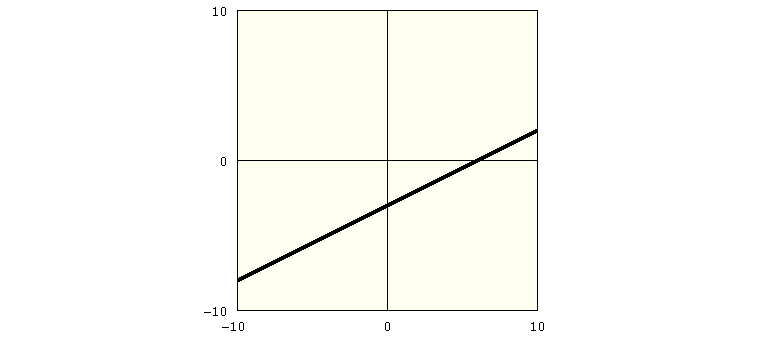
\includegraphics[scale=0.5]{1.png}

\newpage

\noindent
Now suppose that we want to draw the graph
with a different $m$.
We could type in everything all over again, but it would be easier
in the long run to write a script.
Then we can go back and quickly change $m$ and $b$ as many times as we want.

\medskip
\noindent
To prepare a script, click on the Edit Script button.
Then enter the script commands, one per line.

\medskip
{\tt y=m*x+b}

{\tt m=1/2}

{\tt b=-3}

{\tt draw(y)}

\medskip
\noindent
Next, click on the Run Script button to see the graph.

\medskip
\noindent
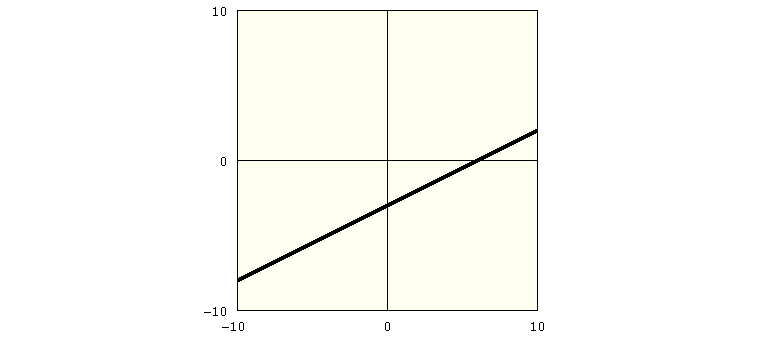
\includegraphics[scale=0.5]{1.png}

\medskip
\noindent
Eigenmath runs a script by stepping through it line by line.
Each line is evaluated just like a regular command.
This continues until the end of the script is reached.
After the script runs, you can click Edit Script and go back and change something.

\medskip
\noindent
It should also be pointed out that Eigenmath automatically does a clear before
running a script.

\newpage

%\section*{Draw}
$draw(f,x)$ draws a graph of the function $f$ of $x$.
The second argument can be omitted when the dependent variable
is literally $x$ or $t$.
The vectors $xrange$ and $yrange$ control the scale of the graph.

\medskip
\verb$draw(x^2)$

\medskip
\begin{center}
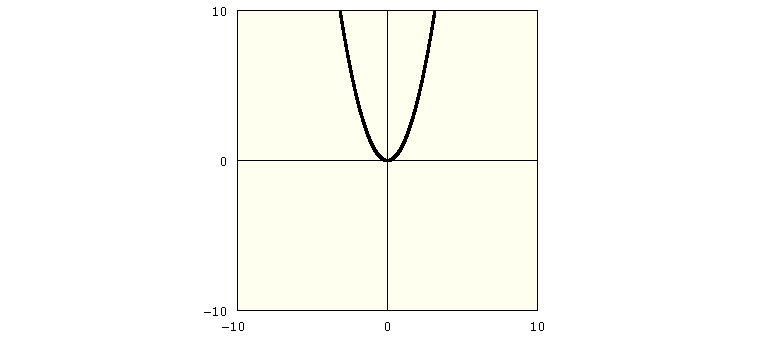
\includegraphics[scale=0.4]{parabola.png}
\end{center}

\verb$xrange=(-1,1)$

\verb$yrange=(0,2)$

\verb$draw(x^2)$

\medskip
\begin{center}
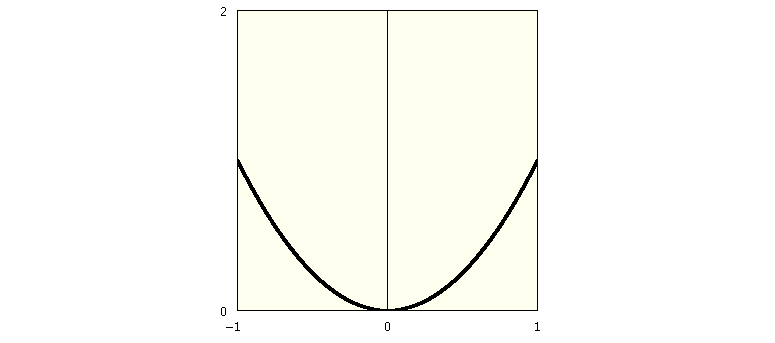
\includegraphics[scale=0.4]{parabola2.png}
\end{center}

\verb$clear$

\medskip
\noindent
The clear command (or a click of the Clear button)
resets $xrange$ and $yrange$.
This needs to be done so that the next graph
appears as shown.

\newpage

\noindent
Parametric drawing occurs when a function returns a vector.
The vector $trange$ controls the parameter range.
The default range is $(-\pi,\pi)$.

\medskip
\verb$f=(cos(t),sin(t))$

\verb$draw(5*f)$

\medskip
\begin{center}
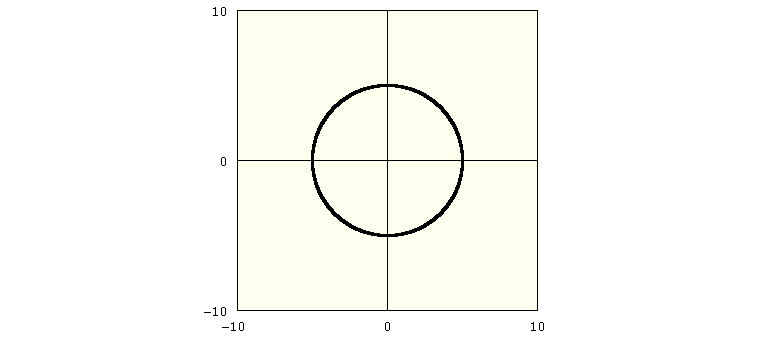
\includegraphics[scale=0.4]{circle.png}
\end{center}

\verb$trange=(0,pi/2)$

\verb$draw(5*f)$

\medskip
\begin{center}
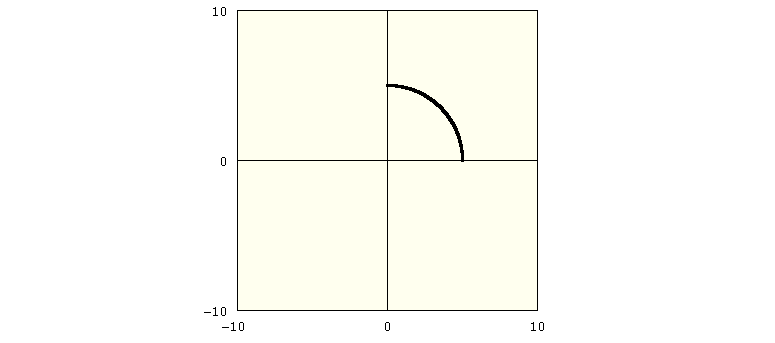
\includegraphics[scale=0.4]{circle2.png}
\end{center}

\newpage

\noindent
Here are a couple of interesting curves and the code for drawing them.
First is a lemniscate.

\medskip
\verb$clear$

\verb$X=cos(t)/(1+sin(t)^2)$

\verb$Y=sin(t)*cos(t)/(1+sin(t)^2)$

\verb$draw(5*(X,Y))$

\medskip
\begin{center}
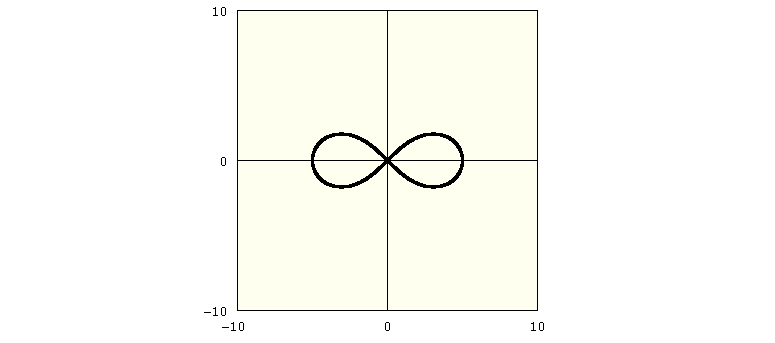
\includegraphics[scale=0.4]{lemniscate.png}
\end{center}

\medskip
\noindent
Next is a cardioid.

\medskip
\verb$r=(1+cos(t))/2$

\verb$u=(cos(t),sin(t))$

\verb$xrange=(-1,1)$

\verb$yrange=(-1,1)$

\verb$draw(r*u)$

\medskip
\begin{center}
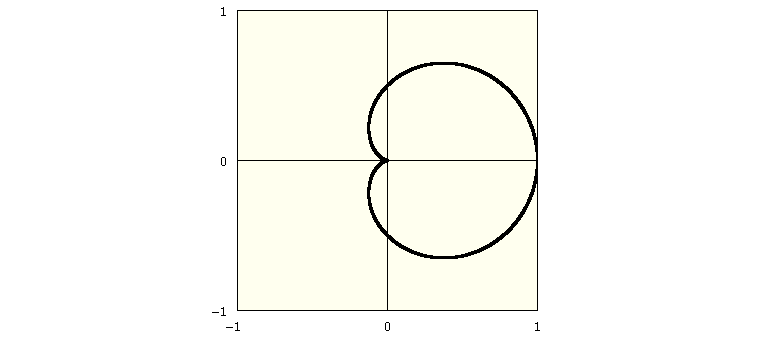
\includegraphics[scale=0.4]{cardioid.png}
\end{center}



\chapter{Draw}

\newpage

\noindent
$draw(f,x)$ draws a graph of the function $f$ of $x$.
The second argument can be omitted when the dependent variable
is literally $x$ or $t$.
The vectors $xrange$ and $yrange$ control the scale of the graph.

\medskip
\verb$draw(x^2)$

\medskip
\noindent
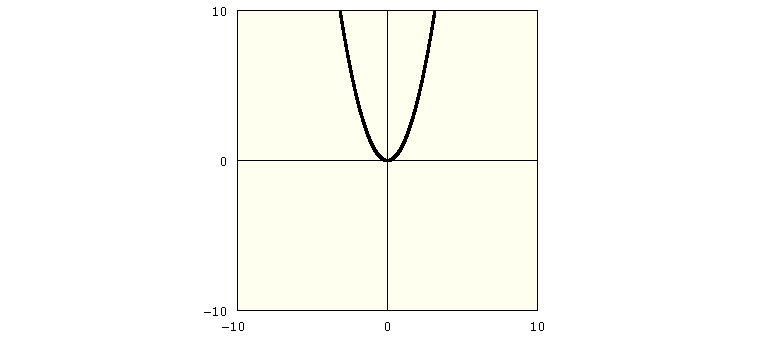
\includegraphics[scale=0.5]{parabola.png}

\verb$xrange=(-1,1)$

\verb$yrange=(0,2)$

\verb$draw(x^2)$

\medskip
\noindent
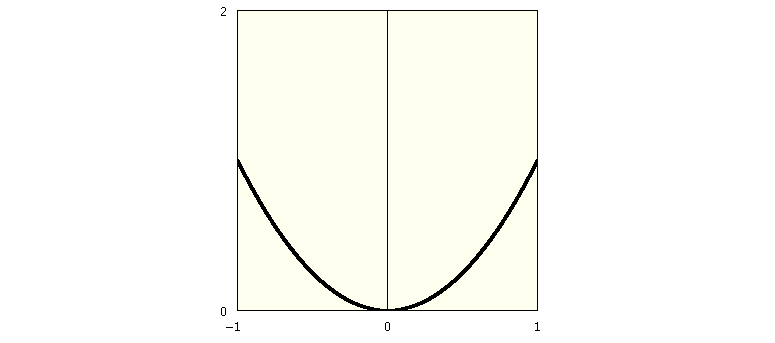
\includegraphics[scale=0.5]{parabola2.png}

\verb$clear$

\medskip
\noindent
The clear command (or a click of the Clear button)
resets $xrange$ and $yrange$.
This needs to be done so that the next graph
appears as shown.

\newpage

\noindent
Parametric drawing occurs when a function returns a vector.
The vector $trange$ controls the parameter range.
The default range is $(-\pi,\pi)$.

\medskip
\verb$f=(cos(t),sin(t))$

\verb$draw(5*f)$

\medskip
\noindent
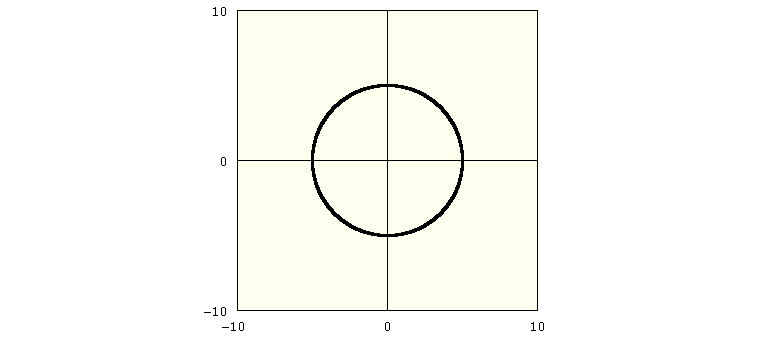
\includegraphics[scale=0.5]{circle.png}

\verb$trange=(0,pi/2)$

\verb$draw(5*f)$

\medskip
\noindent
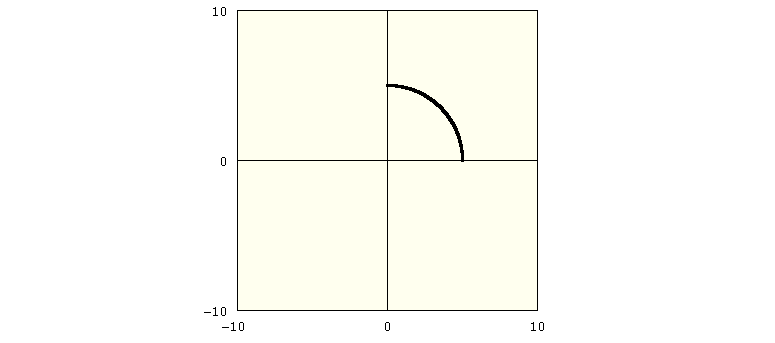
\includegraphics[scale=0.5]{circle2.png}

\newpage

\noindent
Here are a couple of interesting curves and the code for drawing them.
First is a lemniscate.

\medskip
\verb$clear$

\verb$X=cos(t)/(1+sin(t)^2)$

\verb$Y=sin(t)*cos(t)/(1+sin(t)^2)$

\verb$draw(5*(X,Y))$

\medskip
\noindent
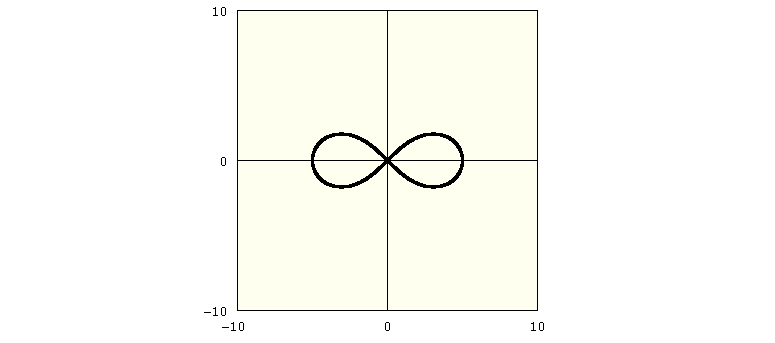
\includegraphics[scale=0.5]{lemniscate.png}

\medskip
\noindent
Next is a cardioid.

\medskip
\verb$r=(1+cos(t))/2$

\verb$u=(cos(t),sin(t))$

\verb$xrange=(-1,1)$

\verb$yrange=(-1,1)$

\verb$draw(r*u)$

\medskip
\noindent
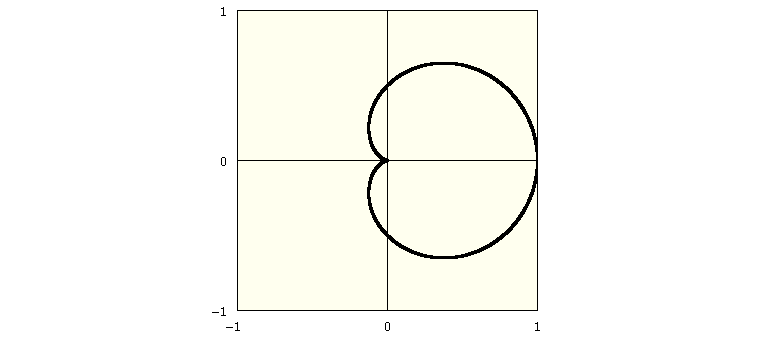
\includegraphics[scale=0.5]{cardioid.png}

\newpage

\chapter{Linear Algebra}

$dot$ is used to multiply vectors and matrices.
The following example shows how to use $dot$ and $inv$ to solve for
$\bf X$ in $\bf AX=B$.

\medskip
{\tt A=((3.8,7.2),(1.3,-0.9))}

{\tt B=(16.5,-22.1)}

{\tt X=dot(inv(A),B)}

{\tt X}

$$\left(\matrix{-11.2887\cr8.24961}\right)$$

\medskip
\noindent
One might wonder why the $dot$ function is necessary.
Why not simply use $X=inv(A)*B$ like scalar multiplication?
The reason is that the software normally reorders factors internally to optimize processing.
For example, $inv(A)*B$ in symbolic form is changed to $B*inv(A)$ internally.
Since the dot product is non-commutative, this reordering would give the wrong result.
Using a function to do the multiply avoids the problem because
function arguments are not reordered.

\medskip
\noindent
It should be noted that $dot$ can have more than two arguments.
For example, $dot(A,B,C)$ can be used for the dot product of three tensors.

\newpage

\label{adj}

\noindent
The following example demonstrates the relation
${\bf A}^{-1}=\mathop{\rm adj}{\bf A}/\mathop{\rm det}{\bf A}$.

\medskip
\verb$A=((a,b),(c,d))$

\medskip
\verb$inv(A)$
$$\left(\matrix{
\displaystyle{d\over ad-bc} & \displaystyle{-{b\over ad-bc}}\cr
\cr
\displaystyle{-{c\over ad-bc}} & \displaystyle{a\over ad-bc}\cr
}\right)$$

\medskip
\verb$adj(A)$
$$\left(\matrix{
d & -b\cr
-c & a\cr
}\right)$$

\medskip
\verb$det(A)$
$$ad-bc$$

\medskip
\verb$inv(A)-adj(A)/det(A)$
$$\left(\matrix{
0 & 0\cr
0 & 0\cr
}\right)$$

\medskip
\noindent
Sometimes a calculation will be simpler if it can be reorganized to use adj instead of inv.
The main idea is to try to prevent the determinant from appearing as a divisor.
For example, suppose for matrices $\bf A$ and $\bf B$ you want to check that
$${\bf A}-{\bf B}^{-1}=0$$
Depending on the complexity of $\mathop{\rm det}\bf B$, the software
may not be able to find a simplification that yields zero.
Should that occur, the following alternative can be tried.
$$(\mathop{\rm det}{\bf B})\cdot{\bf A}-\mathop{\rm adj}{\bf B}=0$$

\newpage

\label{cofactor}

\noindent
The adjunct of a matrix is related to the cofactors as follows.

\medskip
\verb$A=((a,b),(c,d))$

\medskip
\verb$C=((0,0),(0,0))$

\medskip
%\verb$for(i,1,2,for(j,1,2,C[i,j]=cofactor(A,i,j)))$
\verb$C[1,1]=cofactor(A,1,1)$

\verb$C[1,2]=cofactor(A,1,2)$

\verb$C[2,1]=cofactor(A,2,1)$

\verb$C[2,2]=cofactor(A,2,2)$

\medskip
\verb$C$
$$C=\left(\matrix{d&-c\cr -b&a}\right)$$

\medskip
\verb$adj(A)-transpose(C)$
$$\left(\matrix{0&0\cr0&0\cr}\right)$$

\newpage

\chapter{Derivative}

\label{d}

\noindent
$d(f,x)$ returns the derivative of $f$ with respect to $x$.
The $x$ can be omitted for expressions in $x$.

\medskip
\verb$d(x^2)$
$$2x$$

\bigskip
\noindent
The following table summarizes the various ways to obtain multiderivatives.

\begin{center}
\begin{tabular}{cllllll}
%& & & & {\it alternate form} \\
%\\
$\displaystyle{\partial^2f\over\partial x^2}$ & & \verb$d(f,x,x)$ & & \verb$d(f,x,2)$ \\
\\
$\displaystyle{\partial^2f\over\partial x\,\partial y}$ & & \verb$d(f,x,y)$ \\
\\
$\displaystyle{\partial^{m+n+\cdot\cdot\cdot} f\over\partial x^m\,\partial y^n\cdots}$ & &
\verb$d(f,x,...,y,...)$ & & \verb$d(f,x,m,y,n,...)$ \\
\end{tabular}
\end{center}

%\medskip
%\verb$r=sqrt(x^2+y^2)$

%\verb$d(r,x,y)$
%$${-{xy\over(x^2+y^2)^{3/2}}}$$

\newpage

\noindent
The gradient of $f$ is obtained by using a vector for $x$ in $d(f,x)$.

\medskip
\verb$r=sqrt(x^2+y^2)$

\verb$d(r,(x,y))$
$$\left(\matrix{
\displaystyle{{x\over(x^2+y^2)^{1/2}}}\cr
\cr
\displaystyle{{y\over(x^2+y^2)^{1/2}}}\cr
}\right)$$

\medskip
\noindent
The $f$ in $d(f,x)$ can be a tensor function.
Gradient raises the rank by one.

\medskip
\verb$F=(x+2y,3x+4y)$

\verb$X=(x,y)$

\verb$d(F,X)$
$$\left(\matrix{1&2\cr3&4}\right)$$

\newpage

\noindent
The function $f$ in $d(f)$ does not have to be defined.
It can be a template function with just a name and an argument list.
Eigenmath checks the argument list to figure out what to do.
For example, $d(f(x),x)$ evaluates to itself because $f$ depends on $x$.
However, $d(f(x),y)$ evaluates to zero because $f$ does not depend on $y$.

\medskip
\verb$d(f(x),x)$
$$\partial(f(x),x)$$

\verb$d(f(x),y)$
$$0$$

\verb$d(f(x,y),y)$
$$\partial(f(x,y),y)$$

\verb$d(f(),t)$
$$\partial(f(),t)$$

\medskip
\noindent
As the final example shows, an empty argument list causes
$d(f)$ to always evaluate to itself, regardless
of the second argument.

\medskip
\noindent
Template functions are useful for experimenting with differential forms.
For example, let us check the identity
$$\mathop{\rm div}(\mathop{\rm curl}{\bf F})=0$$
for an arbitrary vector function $\bf F$.

\medskip
\verb$F=(F1(x,y,z),F2(x,y,z),F3(x,y,z))$

\verb$curl(U)=(d(U[3],y)-d(U[2],z),d(U[1],z)-d(U[3],x),d(U[2],x)-d(U[1],y))$

\verb$div(U)=d(U[1],x)+d(U[2],y)+d(U[3],z)$

\verb$div(curl(F))$
$$0$$

\newpage

\chapter{Integral}

\label{integral}

\noindent
$integral(f,x)$ returns the integral of $f$ with respect to $x$.
The $x$ can be omitted for expressions in $x$.
A multi-integral can be obtained by extending the argument list.

\medskip
\verb$integral(x^2)$
$${1\over3}x^3$$

\verb$integral(x*y,x,y)$
$${1\over4}x^2y^2$$

\newpage

\noindent
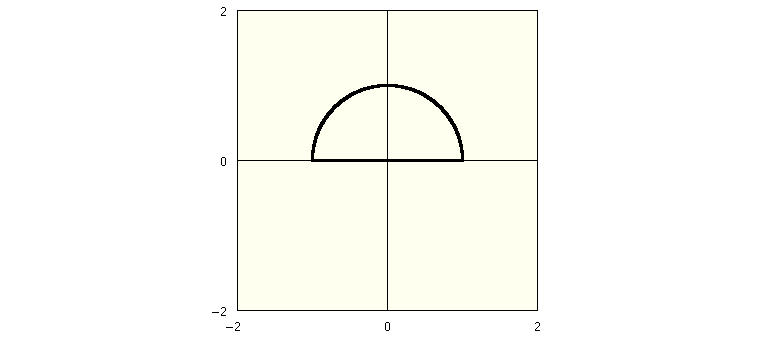
\includegraphics[scale=0.5]{semicircle.png}

\medskip
\noindent
$defint(f,x,a,b,\ldots)$
computes the definite integral of $f$ with respect to $x$ evaluated from $a$ to $b$.
The argument list can be extended for multiple integrals.

\medskip
\noindent
The following example computes the integral of $f=x^2$
over the domain of a semicircle.
For each $x$ along the abscissa, $y$ ranges from 0 to $\sqrt{1-x^2}$.

\medskip
\verb$defint(x^2,y,0,sqrt(1-x^2),x,-1,1)$

$${1\over8}\pi$$

\medskip
\noindent
As an alternative, the $eval$ function can be used to compute a definite integral step by step.

\medskip
\verb$I=integral(x^2,y)$

\verb$I=eval(I,y,sqrt(1-x^2))-eval(I,y,0)$

\verb$I=integral(I,x)$

\verb$eval(I,x,1)-eval(I,x,-1)$
$${1\over8}\pi$$

\newpage

\noindent
The following example demonstrates a technique for computing
a line integral when the path is already parameterized.
The task at hand is to compute\footnote{
From a problem in {\it Advanced Calculus} by Wilfred Kaplan.}
$$\int_C z\,dx+x\,dy+y\,dz$$
where $C$ is the path
$$x=2t+1,\qquad y=t^2,\qquad z=1+t^3,\qquad 0\le t\le 1$$
The main idea is that we can rewrite the integrand with the following substitutions.
$$dx=\left({dx\over dt}\right)dt,\qquad
dy=\left({dy\over dt}\right)dt,\qquad
dz=\left({dz\over dt}\right)dt$$
Therefore in Eigenmath we have

\medskip
\verb$x=2t+1$

\verb$y=t^2$

\verb$z=1+t^3$

\verb$f=z*d(x,t)+x*d(y,t)+y*d(z,t)$

\verb$I=integral(f,t)$

\verb$eval(I,t,1)-eval(I,t,0)$

$$163\over30$$

\newpage

% surface area

\newpage

\noindent
Let $S$ be a surface parameterized by $x$ and $y$.
That is, let $S=(x,y,z)$ where $z=f(x,y)$.
The tangent lines at a point on $S$ form a tiny parallelogram.
The area $a$ of the parallelogram is given by the magnitude of the cross product.
$$a=\left|{\partial S\over\partial x}\times{\partial S\over\partial y}\right|$$
By summing over all the parallelograms we obtain the total surface area $A$.
Hence
$$A=\int\!\!\!\int dA=\int\!\!\!\int a\,dx\,dy$$
The following example computes the surface area of a unit disk
parallel to the $xy$ plane.

\medskip
\verb$z=2$

\verb$S=(x,y,z)$

\verb$a=abs(cross(d(S,x),d(S,y)))$

\verb$defint(a,y,-sqrt(1-x^2),sqrt(1-x^2),x,-1,1)$

$$\pi$$

\medskip
\noindent
The result is $\pi$, the area of a unit circle, which is what we expect.
The following example computes the surface area of $z=x^2+2y$ over
a unit square.

\medskip
\verb$z=x^2+2y$

\verb$S=(x,y,z)$

\verb$a=abs(cross(d(S,x),d(S,y)))$

\verb$defint(a,x,0,1,y,0,1)$

$${3\over2}+{5\over8}\log(5)$$

\medskip
\noindent
As a practical matter, $f(x,y)$ must be very simple in order
for Eigenmath to solve the double integral.

\newpage

\noindent
Find the area of the spiral ramp defined by\footnote{
Williamson and Trotter, {\it Multivariable Mathematics,} p. 598.}
$$S=\left(\matrix{u\cos v\cr u\sin v\cr v}\right),\qquad 0\le u\le1,\qquad 0\le v\le3\pi$$
In this example, the coordinates $x$, $y$ and $z$ are all
functions of an independent parameter space.

\medskip
\verb$x=u*cos(v)$

\verb$y=u*sin(v)$

\verb$z=v$

\verb$S=(x,y,z)$

\verb$a=abs(cross(d(S,u),d(S,v)))$

\verb$defint(a,u,0,1,v,0,3pi)$

$${3\over2}\pi\log(1+2^{1/2})+{3\pi\over2^{1/2}}$$

\verb$float$

$$10.8177$$



\newpage

\chapter{Complex Numbers}

\noindent
When Eigenmath starts up, it defines the symbol $i$ as $i=\sqrt{-1}$.
Other than that, there is nothing special about $i$.
It is just a regular symbol that can be redefined and used for some other purpose if need be.

\medskip
\noindent
Complex quantities can be entered in rectangular or polar form.

\medskip
\verb$a+i*b$
$$a+ib$$

\verb$exp(i*pi/3)$
$$\exp({1\over3}i\pi)$$

\medskip
\noindent
Converting to rectangular or polar coordinates simplifies mixed forms.

\medskip
\verb$A=1+i$

\verb$B=sqrt(2)*exp(i*pi/4)$

\verb$A-B$
$$1+i-2^{1/2}\exp({1\over4}i\pi)$$

\verb$rect$
$$0$$

\newpage

\noindent
Rectangular complex quantities, when raised to a power, are multiplied out.

\medskip
\verb$(a+i*b)^2$
$$a^2-b^2+2iab$$

\medskip
\noindent
When $a$ and $b$ are numerical and the power is negative, the evaluation is done as follows.
$$(a+ib)^{-n}=\left[{a-ib\over(a+ib)(a-ib)}\right]^n=\left[{a-ib\over a^2+b^2}\right]^n$$
This removes $i$ from the denominator.
%For $n=1$ we have
%$${1\over a+ib}={a-ib\over a^2+b^2}$$
Here are a few examples.

\medskip
\verb$1/(2-i)$
$${2\over5}+{1\over5}i$$

\verb$(-1+3i)/(2-i)$
$$-1+i$$

\newpage

\chapter{List of Eigenmath Functions}

\section*{abs}
abs($x$) returns the absolute value or vector length of $x$.
The mag function should be used for complex $x$.

\medskip
{\tt P=(x,y)}

{\tt abs(P)}

$$(x^2+y^2)^{1/2}$$

\section*{adj}
adj($m$) returns the adjunct of matrix $m$.
Please see page \pageref{adj} for an example.

\section*{and}
and($a,b,\ldots$) returns the logical ``and'' of predicate expressions.

\section*{arccos}
arccos($x$) returns the inverse cosine of $x$.

\section*{arccosh}
arccosh($x$) returns the inverse hyperbolic cosine of $x$.

\section*{arcsin}
arcsin($x$) returns the inverse sine of $x$.

\section*{arcsinh}
arcsinh($x$) returns the inverse hyperbolic sine of $x$.

\section*{arctan}
arcttan($x$) returns the inverse tangent of $x$.

\section*{arctanh}
arctanh($x$) returns the inverse hyperbolic tangent of $x$.

\section*{arg}
arg($z$) returns the angle of complex $z$.

\section*{ceiling}
ceiling($x$) returns the smallest integer not less than $x$.

\section*{check}
check($x$) In a script, if the predicate $x$ is true then continue, else stop.

\section*{choose}
choose($n,k$) returns $\displaystyle\left({n \atop k}\right)$

\section*{circexp}
circexp($x$) returns expression $x$ with circular functions converted
to exponential forms.
Sometimes this will simplify an expression.

\section*{coeff}
coeff($p,x,n$) returns the coefficient of $x^n$ in polynomial $p$.

\section*{cofactor}
cofactor($m,i,j$) returns of the cofactor of matrix $m$ with respect to row $i$ and column $j$.
Please see page \pageref{cofactor} for an example.

\section*{conj}
conj($z$) returns the complex conjugate of $z$.

\section*{contract}
contract($a,i,j$) returns tensor $a$ summed over indices $i$ and $j$.

\section*{cos}
cos($x$) returns the cosine of $x$.
%If $x$ is a floating point number then $\cos(x)$ is evaluated numerically.

\section*{cosh}
cosh($x$) returns the hyperbolic cosine of $x$.

\section*{d}
d($f,x$) returns the derivative of $f$ with respect to $x$.
Please see page \pageref{d} for additional details.

\section*{defint}
defint($f,x,a,b,\ldots$)
returns the definite integral of $f$ with respect to $x$ evaluated from $a$ to $b$.
The argument list can be extended for multiple integrals.
For example, $d(f,x,a,b,y,c,d)$.

\section*{deg}
deg($p,x$) returns the degree of polynomial $p$ in $x$.

\section*{denominator}
denominator($x$) returns the denominator of expression $x$.

\section*{det}
det($m$) returns the determinant of matrix $m$.

\section*{display}
display($x$) evaluates expression $x$ and displays the result.
Useful for printing from inside a ``for'' loop.

\section*{do}
do($a,b,\ldots$) evaluates the argument list from left to right.
Returns the result of the last argument.

\section*{dot}
dot($a,b,\ldots$) returns the dot product of tensors.

\section*{draw}
draw($f,x$) draws the function $f$ with respect to $x$.

\section*{erf}
erf($x$) returns the error function of $x$.

\section*{erfc}
erf($x$) returns the complementary error function of $x$.

\section*{eval}
eval($f,x,n$) returns $f$ evaluated at $x=n$.
Please see page \pageref{integral} for an example.

\section*{exp}
exp($x$) returns $e^x$.

\section*{expcos}
expcos($x$) returns the cosine of $x$ in exponential form.

\medskip
{\tt expcos(x)}

$${1\over2}\exp(-ix)+{1\over2}\exp(ix)$$

\section*{expsin}
expsin($x$) returns the sine of $x$ in exponential form.

\medskip
{\tt expsin(x)}

$${1\over2}i\exp(-ix)-{1\over2}i\exp(ix)$$

\section*{factor}
factor($n$) factors the integer $n$.

\medskip
{\tt factor(12345)}

$$3\times 5\times 823$$

\medskip
\noindent
factor($p,x$) factors polynomial $p$ in $x$.
The last argument can be omitted for polynomials in $x$.

\medskip
{\tt factor(125*x{\char94}3-1)}

$$(5x-1)(25x^2+5x+1)$$

\section*{factorial}
Example:

\medskip
{\tt 10!}

$$3628800$$

\section*{filter}
filter($f,a,b,\ldots$) returns $f$ with terms involving $a$, $b$, etc. removed.

\medskip
{\tt 1/a+1/b+1/c}

$${1\over a}+{1\over b}+{1\over c}$$

{\tt filter(last,a)}

$${1\over b}+{1\over c}$$

\section*{float}
float($x$) converts $x$ to a floating point value.

\medskip
{\tt sum(n,0,20,(-1/2){\char94}n)}

$$699051\over1048576$$

{\tt float(last)}

$$0.666667$$

\section*{floor}
floor($x$) returns the largest integer not greater than $x$.

\section*{for}
for($i,j,k,a,b,\ldots$) For $i$ equals $j$ through $k$ evaluate $a$, $b$, etc.

\medskip
{\tt x=0}

{\tt y=2}

{\tt for(k,1,9,x=sqrt(2+x),y=2*y/x)}

{\tt float(y)}

$$3.14159$$

\section*{gcd}
gcd($a,b,\ldots$) returns the greatest common divisor.

\section*{hermite}
hermite($x,n$) returns the $n$th Hermite polynomial in $x$.

\section*{hilbert}
hilbert($n$) returns a Hilbert matrix of order $n$.

\section*{imag}
imag($z$) returns the imaginary part of complex $z$.

\section*{inner}
inner($a,b,\ldots$) returns the inner product of tensors.
Same as the dot product.

\section*{integral}
integral($f,x$) returns the integral of $f$ with respect to $x$.
Please see page \pageref{integral} for additional details.

\section*{inv}
inv($m$) returns the inverse of matrix $m$.

\section*{isprime}
isprime($n$) returns 1 if $n$ is prime, zero otherwise.

\medskip
{\tt isprime(2{\char94}53-111)}

$$1$$

\section*{laguerre}
laguerre($x,n,a$) returns the $n$th Laguerre polynomial in $x$.
If $a$ is omitted then $a=0$ is used.

\section*{lcm}
lcm($a,b,\ldots$) returns the least common multiple.

\section*{legendre}
legendre($x,n,m$) returns the $n$th Legendre polynomial in $x$.
If $m$ is omitted then $m=0$ is used.

\section*{log}
log($x$) returns the natural logarithm of $x$.

\section*{mag}
mag($z$) returns the magnitude of complex $z$.

\section*{mod}
mod($a,b$) returns the remainder of $a$ divided by $b$.

\section*{not}
not($x$) negates the result of predicate expression $x$.

\section*{numerator}
numerator($x$) returns the numerator of expression $x$.
%\begin{itemize}
%\item[$\scriptstyle1$]{\tt numerator(a/b+b/a)}
%\item[$\scriptstyle2$]\hspace{50pt} $a^2+b^2$
%\end{itemize}

\section*{or}
or($a,b,\ldots$) returns the logical ``or'' of predicate expressions.

\section*{outer}
outer($a,b,\ldots$) returns the outer product of tensors.

\section*{polar}
polar($z$) converts complex $z$ to polar form.

\section*{prime}
prime($n$) returns the $n$th prime number, $1\le n\le10{,}000$.

\section*{print}
print($x$) evaluates expression $x$ and displays the result in typewriter style.
Useful for printing from inside a ``for'' loop.

\section*{product}
product($i,j,k,f$) returns $\displaystyle\prod_{i=j}^k f$

\section*{quote}
quote($x$) returns expression $x$ unevaluated.

\section*{quotient}
quotient($p,q,x$) returns the quotient of polynomials in $x$.

\section*{rank}
rank($a$) returns the number of indices that tensor $a$ has.
A scalar has no indices so its rank is zero.

\section*{rationalize}
rationalize($x$) puts everything over a common denominator.

\medskip
{\tt rationalize(a/b+b/a)}

$$a^2+b^2\over ab$$

\section*{real}
real($z$) returns the real part of complex $z$.

\section*{rect}
rect($z$) returns complex $z$ in rectangular form.

\section*{roots}
roots($p,x$) returns the values of $x$ such that the polynomial $p(x)=0$.
The polynomial should be factorable over integers.

\section*{simplify}
simplify($x$) returns $x$ in a simpler form.

\section*{sin}
sin($x$) returns the sine of $x$.

\section*{sinh}
sinh($x$) returns the hyperbolic sine of $x$.

\section*{sqrt}
sqrt($x$) returns the square root of $x$.

\section*{stop}
In a script, it does what it says.

\section*{subst}
subst($a,b,c$) substitutes $a$ for $b$ in $c$ and returns the result.

\section*{sum}
sum($i,j,k,f$) returns $\displaystyle\sum_{i=j}^k f$

\section*{tan}
tan($x$) returns the tangent of $x$.

\section*{tanh}
tanh($x$) returns the hyperbolic tangent of $x$.

\section*{taylor}
taylor($f,x,n,a$) returns the Taylor expansion of $f$ of $x$ at $a$.
The argument $n$ is the degree of the expansion.
If $a$ is omitted then $a=0$ is used.

\medskip
{\tt taylor(1/cos(x),x,4)}

$${5\over24}x^4+{1\over2}x^2+1$$

\section*{test}
test($a,b,c,d,\ldots$)
If $a$ is true then $b$ is returned else if $c$ is true then $d$ is returned, etc.
If the number of arguments is odd then the last argument is returned when all else fails.

\section*{trace}
trace($m$) returns the trace of matrix $m$.

\section*{transpose}
transpose($a,i,j$) returns the transpose of tensor $a$ with respect to indices $i$ and $j$.
If $i$ and $j$ are omitted then 1 and 2 are used.
Hence a matrix can be transposed with a single argument.

\medskip
{\tt A=((a,b),(c,d))}

{\tt transpose(A)}

$$\left[\matrix{a & c\cr b & d\cr}\right]$$

\section*{unit}
unit($n$) returns an $n\times n$ identity matrix.

\medskip
{\tt unit(2)}

$$\left(\matrix{1&0\cr0&1\cr}\right)$$

\section*{zero}
zero($i,j,\ldots$) returns a null tensor with dimensions $i$, $j$, etc.
Useful for creating a tensor and then setting the component values.
See page \pageref{example2}.

\newpage

\chapter{Examples}

\newpage

\section*{Example 1}
Fran\c cois Vi\`ete was the first to discover an exact formula for $\pi$.
Here is his formula.
\begin{displaymath}
{2\over\pi}={\sqrt2\over2}\times{\sqrt{2+\sqrt2}\over2}\times
{\sqrt{2+\sqrt{2+\sqrt2}}\over2}\times\cdots
\end{displaymath}
%We can flip it around and write the formula like this.
%\begin{displaymath}
%\pi=2\times{2\over\sqrt2}\times{2\over\sqrt{2+\sqrt2}}\times
%{2\over\sqrt{2+\sqrt{2+\sqrt2}}}\times\cdots
%\end{displaymath}
Let $a_0=0$ and $a_{n}=\sqrt{2+a_{n-1}}$.
Then we can write
\begin{displaymath}
{2\over\pi}={a_1\over2}\times{a_2\over2}\times
{a_3\over2}\times\cdots
\end{displaymath}
%
Solving for $\pi$ we have
\begin{displaymath}
\pi=2\times{2\over a_1}\times{2\over a_2}\times{2\over a_3}\times\cdots=2\prod_{k=1}^\infty
{2\over a_k}
\end{displaymath}
%
Let us now use Eigenmath to compute $\pi$ according to Vi\`ete's formula.
Of course, we cannot calculate all the way out to infinity, we have to stop somewhere.
It turns out that nine factors are just enough to get six digits of accuracy.

\medskip
\verb$a(n)=test(n=0,0,sqrt(2+a(n-1)))$

\verb$float(2*product(k,1,9,2/a(k)))$

$$3.14159$$

\medskip
\noindent
The function $a(n)$ calls itself $n$ times so overall there are
54 calls to $a(n)$.
By using a different algorithm with temporary variables, we can get the
answer in just nine steps.

\medskip
\verb$a=0$

\verb$b=2$

\verb$for(k,1,9,a=sqrt(2+a),b=b*2/a)$

\verb$float(b)$

$$3.14159$$

\newpage

\label{example2}

\section*{Example 2}
The curl of a vector function can be expressed in tensor form as
$$\mathop{\rm curl}{\bf F}=\epsilon_{ijk}\,{\partial F_k\over\partial x_j}$$
where $\epsilon_{ijk}$ is the Levi-Civita tensor.
The following script demonstrates that this formula is equivalent
to computing curl the old fashioned way.
First, define $\epsilon_{ijk}$.

\medskip
{\tt
epsilon=zero(3,3,3)

epsilon[1,2,3]=1

epsilon[2,3,1]=1

epsilon[3,1,2]=1

epsilon[3,2,1]=-1

epsilon[1,3,2]=-1

epsilon[2,1,3]=-1
}

\medskip
\noindent
Next, define a generic vector function $\bf F$ and
then compute $A=\epsilon_{ijk}\,\partial F_k/\partial x_j$.
The first summation is over $k$ which corresponds to indices 3 and 4.
The second summation is over $j$ which (with $k$ out of the way)
corresponds to indices 2 and 3.

\medskip
{\tt
F=(FX(),FY(),FZ())

A=outer(epsilon,d(F,(x,y,z)))

A=contract(A,3,4)

A=contract(A,2,3)
}

\medskip
\noindent
Now compute curl the old fashioned way and check for equality.

\medskip
{\tt
B=(

\ d(F[3],y)-d(F[2],z),

\ d(F[1],z)-d(F[3],x),

\ d(F[2],x)-d(F[1],y)

)

\medskip
A-B
}

$$\left(\matrix{0\cr0\cr0}\right)$$

\newpage

\noindent
The following is a variation on the previous script.
The product $\epsilon_{ijk}\,\partial F_k/\partial x_j$
is computed in just one line of code.
In addition, there is an optimization.
The outer product and the first contraction have been replaced with a
dot product.

\medskip
\verb$F=(FX(),FY(),FZ())$

\medskip
\verb$epsilon=zero(3,3,3)$

\verb$epsilon[1,2,3]=1$

\verb$epsilon[2,3,1]=1$

\verb$epsilon[3,1,2]=1$

\verb$epsilon[3,2,1]=-1$

\verb$epsilon[1,3,2]=-1$

\verb$epsilon[2,1,3]=-1$

\medskip
\verb$A=contract(dot(epsilon,d(F,(x,y,z))),2,3)$

\medskip
\verb$B=($

\verb$ d(F[3],y)-d(F[2],z),$

\verb$ d(F[1],z)-d(F[3],x),$

\verb$ d(F[2],x)-d(F[1],y)$

\verb$)$

\medskip
\verb$--Are A and B equal? Subtract to find out.$

\medskip
\verb$A-B$

\end{document}
